%!TEX root = ../../dissertation.tex


\section{Undiscovered City} % (fold)
\label{sec:undiscovered_city}

In \cite{Greuter2003} Stefan Greuter et al. presented a system that generates in real-time pseudo infinite virtual cities which can be interactively explored from a first person perspective. In their approach ``all geometrical components of the city are generated as they are encountered by the user." As shown in the Figure~\ref{fig:viewingRange} only the part of city that is inside the viewing range is generated. This method allows the visualization of massive amounts of geometry, buildings in this case, by generating in real time only the geometry that on sight, and since this subset is usually much smaller than all the geometry this results in huge benefits in performance.

\begin{figure}[htbp]
	\centering
	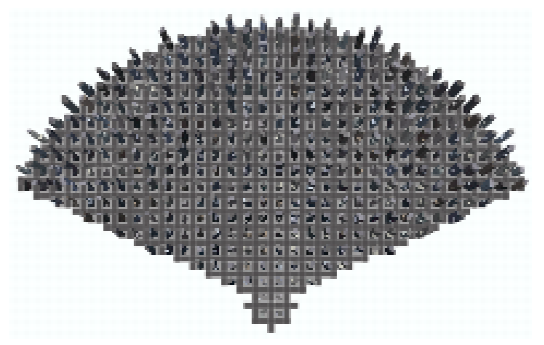
\includegraphics[width=0.85\textwidth]{images/Real-Time-procedural-generation/viewing-range.png}
	\caption{Viewing Range}
	\label{fig:viewingRange}
\end{figure}


The system uses a 2D grid that divide the terrain into square cells. The cells represent proxies for the content that will be procedurally generated. Before the content of each cell is generated, the potential visibility of it is tested, and after that, only the visible cells are filled with content.

Then the roads are created in a uniform grid pattern. This grid does not feel very natural, and with the continuation of the work, this system have become more realistic, with the join of some of the grids to create a less uniform distribution of the buildings.

The buildings within this project are generated with the simple extrusion of regular polygons. This extruded forms are composed to create complex architectural models.


(...)
% section undiscovered_city (end)